 
\section{Model Evaluation}
We evaluate the ability of the network model, testing its performance in different training and testing conditions. We perform the following experiments with two phones: a Redmi 6A smartphone, with a single rear camera with 13 million pixels and digital zoom only, and a HUAWEI P40 Pro, with multiple rear cameras, the telephoto camera(which we use in the experiments) possessing up to 5x optical zooming ability which we will utilize fully in our experiments. 
\subsection{Performance In Controlled Environment}
We train and test the model with the images captured with exactly the same environment parameters, and used Peak Signal to Noise Ratio to evaluate the accuracy of the recovered images(see Table~\ref{table-control} and Fig.~\ref{fig-control}). Moreover, the ultimate goal of our system is the readability of the recovered images, so we also used Optical Character Recognition(OCR) services to evaluate the accuracy. The model with traditional lenses(without optical zoom) is trained and tested at 1~2 meters range, while the one with optical zoom at 5~7.5 meters, at which distance less than 5\% of the characters(only the simplist ones) can be recognized by humans from the photos without the assistance of SR algorithms. The model can achieve an accuracy above 90\% at 1.8m with traditional lenses and 6m with optical zooming lenses. Considering the complexity of Chinese characters, and the assist of context when read by an OCR recognizer, we believe this level of accuracy can provide sufficient data at a shoulder surfing scenario, thus proving the efficiency of our model.
In the optical zoom group the accuracy of the model dropped drastically at 7m distance. Increased distances means less data and less restrictions of the possible outputs, which leads to artifacts(missing or misplaced strokes,etc.). It's the nature of Chinese characters that one mistaken stroke will largely affect its readability, leading to the result that while the pixelwize error rises steadily with the increased distance, the accuracy will experience a drastic drop.

\begin{table}  
\begin{tabular}{c|c|c|c|c} 
Environment & Day,1.4m & Day,1.8m & Night,1.4m & Night,1.8m \\ \hline
PSNR(db) & 14.64 & 12.39 & 10.728 & 10.259 \\ \hline
OCR Accuracy(\%) & 100 & 97 & 95 & 94 \\
\end{tabular} 
\caption{Performance in Controlled Environment}
\label{table-control}
\end{table}

\begin{figure}
 \centering
    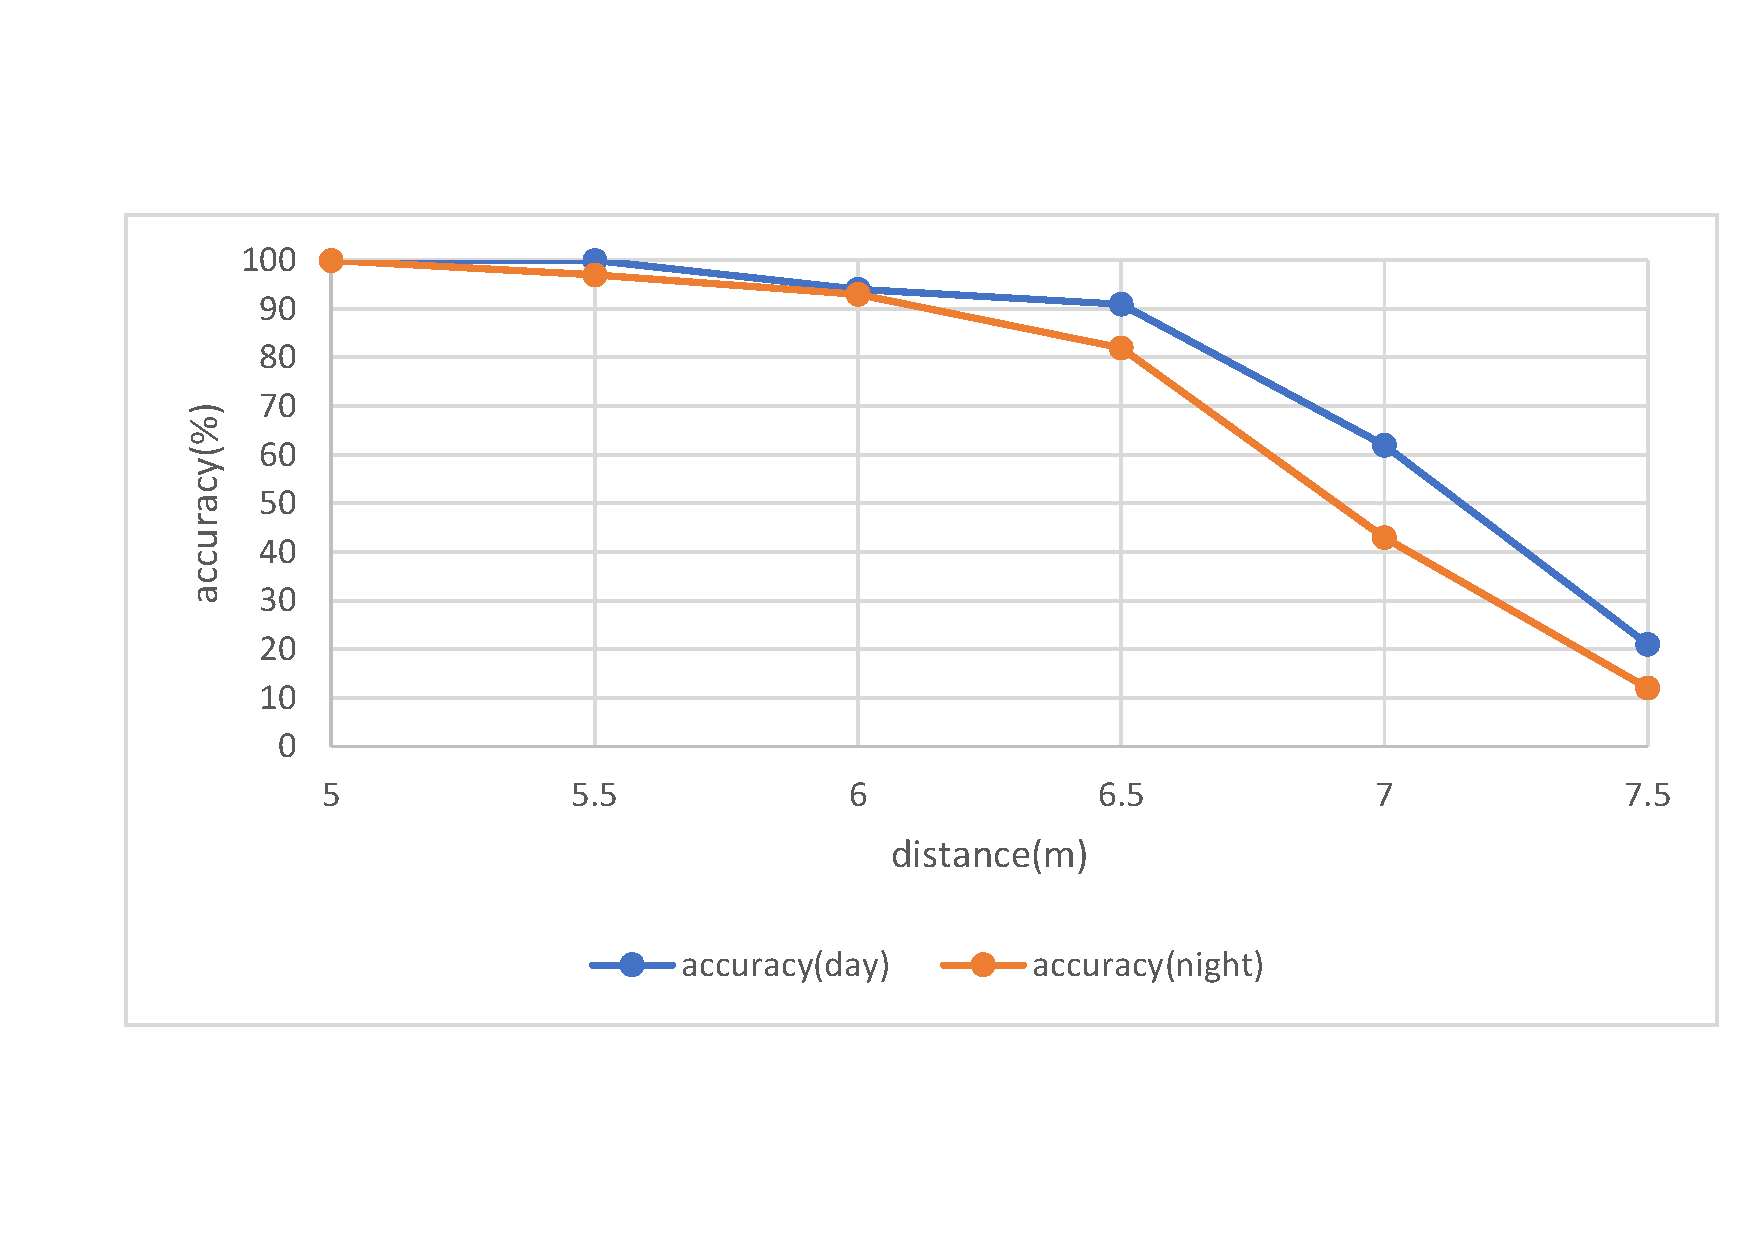
\includegraphics[width=0.5\textwidth]{./pic/distance.pdf}
    \caption{Performance in Controlled Environment(optical zoom lenses)}
    \label{fig-control}
\end{figure}
\subsection{Performance In Random Environment}
We train the model with data captured in different environments, as mentioned before, and test its ability in other environments(see Table~\ref{table-random} and Fig.~\ref{fig-random}). The model achieves an accuracy above 90\% at 1.8m with traditional lenses and 6m with optical zooming lenses. 

\begin{table}  
\begin{tabular}{c|c|c|c|c} 
Environment & Day,1.4m & Day,1.8m & Night,1.4m & Night,1.8m \\ \hline
PSNR(db) & 13.32 & 11.17 & 9.744 & 9.558 \\ \hline
OCR Accuracy(\%) & 100 & 97 & 92 & 85 \\
\end{tabular} 
\caption{Performance in Random Environment(traditional lenses)}
\label{table-random}
\end{table}

\begin{figure}
 \centering
    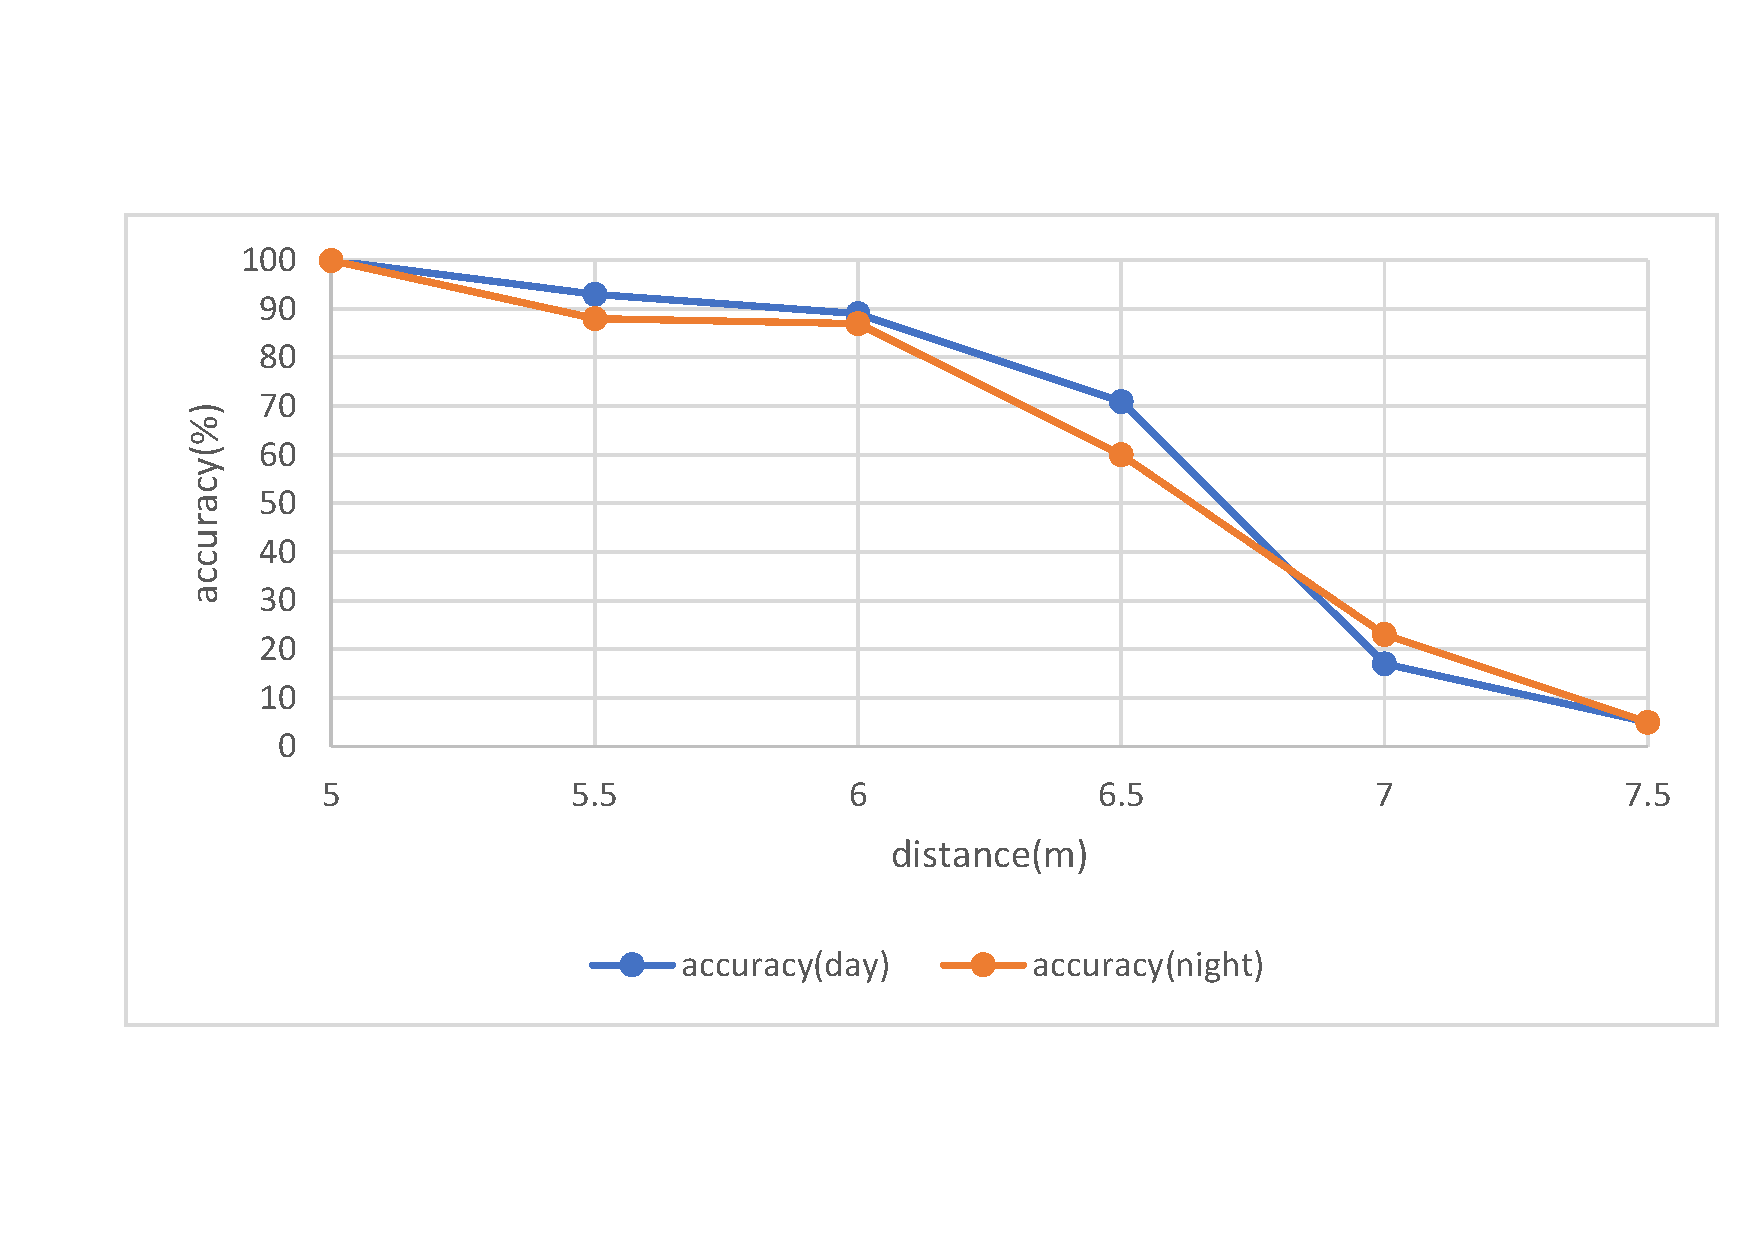
\includegraphics[width=0.5\textwidth]{./pic/distance2.pdf}
    \caption{Performance in Random Environment(optical zoom lenses)}
    \label{fig-random}
\end{figure}
We compare the results to discover the influence of the surrounding environment: The model performs best in daytime and weaker illumination may decrease its ability. Also, the model performs better at closer distances. As the model is trained initially on the 5m group data, it performs expecially well at this distance, while the accuracy at other distances experience certain levels of decrease. Also, similar to the experiments at controlled environments, random artifacts start to encompass OCR compensation, rendering the result images highly unreadable, until at 7.5m distance only the simplist characters can escape from being flooded by noize.

\subsection{Adapting Ability}
We train the model with fewer groups of data, exposing it to fewer variations of environment parameters, and examine the model’s performance in other environments. The results are shown in Table~\ref{table-adapt}.Only the results from the traditional lenses is shown, as the optical zoom lenses group face longer distances and more complex distortions, and with incomplete data the model fails to manage any reasonable reconstruction on the test dataset, resulting in extremely low accuracy in all experiments.

\begin{table*}  
\begin{tabular}{c|c|c|c|c} 
Data & All Data & Night only & 1.2m distance only & Direct angle only \\ \hline
PSNR(db) & 13.32 & 9.17 & 9.94 & 8.84\\ \hline
OCR Accuracy & 100 & 73 & 80 & 52\\
\end{tabular} 
\caption{Adapting Ability}
\label{table-adapt}
\end{table*}

We observed that variations in light and angle parameter in training data is crucial to a robust model. Variations in distance is not so influential to the results, given that the distances are between 1 and 2 meters. Distance changes do not have such a large impact on the size of the characters shown in the images, so that features extracted from a fixed distance might still exist when these characters vary slightly in size. However, if the network is not exposed to angled images during the training process, the rotations and deformations caused by these angles will easily disturb the feature extraction process.

\subsection{Comparison with other architectures}
We train and test other commonly used architectures with the same sets of data and evaluate their results. We chose SRCNN, a commonly used single image SR network, and applied it to each single image before merging the results by pixel-level averageing. We also used a multi-frame version of CNN consisting of 3D convolutional layers, designed for video super resolution(VideoSR). However, as mentioned above, it is very difficult for the single image approaches to utilize information and distinguish the noized and deformed patterns, while VideoSR approaches rely apon consistency between frames, so they fail to give satisfactory results. We used the relatively easy 'daytime 1.2m-distance direct with traditional lenses' group of data for testing. The results are shown in Table~\ref{table-comp}.

\begin{table}  
\begin{tabular}{c|c|c|c} 
Model & Ours & SRCNN & VideoSR \\ \hline
PSNR(db) & 13.32 & 7.690 & 8.403 \\ \hline
OCR Accuracy(\%) & 100 & 10 & 23 \\
\end{tabular} 
\caption{Comparison with other architectures}
\label{table-comp}
\end{table}

\section{System Evaluation}
\subsection{Accuracy}
We build the system on smartphone and evaluate its performance in real-life environments. We experiment with a Redmi 6A smartphone (with a camera of 13 million pixels) for the attacker and a HUAWEI Mate8 smartphone for the victim. As the telephoto cameras can assist the attacker to see clearly at approximately 3m distance without any aid from SR algorithms, we believe it's insignificant to further extend this distance to judge it as a threat to privacy, so that the following experiments are performed with traditional lenses at 1~2m range. We ask 5 human participants to read the reconstructed characters to evaluate the usability of our model. No participants can read the unprocessed images, but all of them can decipher the information on the reconstructed image without much difficulty. The results are shown in Table~\ref{table-accuracy}.

\begin{table*}  
\begin{tabular}{c|c|c|c} 
Scenario & Home & Transport & Theater\\ \hline
Valid images & 20 & 20 & 20\\ \hline
OCR Accuracy(\%) & 95 & 80 & 65\\ \hline
Human Recognition Accuracy(raw data)(\%) & 5 & 0 & 0\\ \hline
Human Recognition Accuracy(processed image)(\%) & 95 & 85 & 70 \\
\end{tabular} 
\caption{Accuracy in different real-life scenarios}
\label{table-accuracy}
\end{table*}

\subsection{Influence of hand tremors}
We ask 5 participants to capture images with handheld smartphones, keeping their hand still to their greatest effort(Handheld camera). We process these images and let them read the results. We compare this performance to the data collected on stationary phones to evaluate the influence of hand tremors.
We also ask participants to hold a smartphone in their hands and read a piece of text, without other additional instructions(Handheld target). The user may freely interact with the phone when reading. We capture images of the phone at the same time to see how our system deal with a moving target screen.The results are shown in Table~\ref{table-tremor}.
\begin{table*}  
\begin{tabular}{c|c|c|c|c} 
Scenario &Stationary & Handheld camera & Handheld target & Handheld camera and target\\ \hline
Valid images & 20 & 19 & 20 & 18\\ \hline
OCR Accuracy(\%) & 95 & 85 & 80 & 80\\ \hline
Human Recognition Accuracy(raw data)(\%) & 5 & 0 & 5 & 5\\ \hline
Human Recognition Accuracy(processed image)(\%) & 95 & 85 & 80 & 85
\end{tabular} 
\caption{Influence of hand tremors}
\label{table-tremor}
\end{table*}

We conclude from the results that hand tremors can impact the performance of our system. Although the edges of the phone are notable marks for image alignment, small shifts in the sub-pixel level will cause blurriness in the results of the networks, lowering the readability of the outputs. 

\subsection{Success rate in different tasks}
We test the success rate of obtaining crucial information when the observed participant perform several tasks on a phone: reading text message, typing text message, entering PIN, and typing password with numbers, English and special characters. The observed participant will turn off the screen of his phone as soon as he/she finishes the task, while the observing participant will observe through our APP, constantly capturing images and processing them to display a real-time and magnified view of the observed phone. For the first two tasks,we ask the observing participant several questions to test if he/she have collected the vital information(e.g. the name or the location mentioned in the text). For the task of recognizing PIN and passwords, we use accuracy per character as a supplementary evaluation metric. The results are shown in Table~\ref{table-task}.

\begin{table*}  
\begin{tabular}{c|c|c|c|c} 
Scenario & Read text & Type text & Enter PIN & Enter complex password\\ \hline
Human Recognition Accuracy(raw image) & 5 & 0 & 0 & 0\\ \hline
Accuracy & 100 & 100 & - & -\\ \hline
Accuracy per character& - & - & 100 & 80\\ 
\end{tabular}
\caption{Success rate in different tasks}
\label{table-task}
\end{table*}

We prove from this experiment that our system functions normally in everyday scenarios and poses a threat to screen privacy.

\subsection{Perceived shoulder surfing susceptibility}
We ask the observed participant to rate the perceived shoulder-surfing susceptibility in these scenario. The attacker will be sitting or standing behind the participant at 1.5m range, pretending to be interacting with their own phone while continuously running the shoulder-surfing APP. None of the participants were alerted by the attacker's behavior and reported suspicion of shoulder-surfing. We believe that our system can enable a malicious attacker to gather large amounts of critical information from the victim while remaining unnoticed.
\section{Limitations}
\subsection{Image Capturing Ability}
Latest models of smartphones can capture images at 10 frames per second in burst mode easily, however, this ability is not common in models 3~4 years old. Heavily used phones also performs less than ideal when capturing images in burst mode. Also, when capturing images the user need to hold their phone as still as possible to avoid motion blur and assist image alignment. The user also has to keep a sharp focus on the target phone.
\subsection{Processing Ability}
To achieve best performance the user needs a phone with strong processing capabilities to run the neural network at real time. As neural networks have been common place in numerous modern APPs, most phones of the latest generation have upgraded their processing ability to run neural networks, but older versions might not possess such processing powers and cannot process images at real-time.
\subsection{Motion and Tremors}
In our experiment we assume the observed user will hold still his/hers phone, and not making interactions too often. However some users may tilt their phones during interactions—especially when typing with one hand. Too much tremor will cause motion blur in captured images and misalignment between frames, thus degrading the result.




